\documentclass[12pt,a4paper]{report}
\usepackage[utf8]{inputenc}
\usepackage{amsmath}
\usepackage{amsfonts}
\usepackage{amssymb}
\usepackage{graphicx}
\usepackage[left=2cm,right=2cm,top=2cm,bottom=2cm]{geometry}
\author{Fahim Masud Choudhury}
\title{Improvement of Handoff Performance in Wireless Mesh Networks}
% arara: indent
\begin{document}
\maketitle
\tableofcontents
\newpage
\begin{center}
\section*{Acknowledgment}
\end{center}
\newpage
\begin{center}
\section*{Abstract}
\end{center}

\chapter{Introduction}
\section{Introduction}
\section{Research Motivation}
\section{Contribution of the Work}
\section{Organization of the Project}

\chapter{Literature Review}

\section{Wireless Mesh Network}
As various wireless networks evolve into the next generation to provide better services, a key technology, wireless mesh networks (WMNs) has emerged recently. In WMNs, nodes are comprised of mesh routers and mesh clients. Each node operates not only as a host but
also as a router, forwarding packets on behalf of other nodes that may not be within direct
wireless transmission range of their destinations. A WMN is dynamically self-organized and self-configured, with the nodes in the network automatically establishing and maintaining
mesh connectivity among themselves. 

Conventional nodes, e.g., desktops, laptops, PDAs, PocketPCs, phones, equipped with
wireless network interface cards (NICs) can be connected directly to wireless mesh routers.
Customers without wireless NICs can access WMNs by connecting to wireless mesh
routers through, for example, Ethernet. Thus, WMNs will greatly help users to be always-
on-line anywhere anytime. Moreover, the gateway/bridge functionalities in mesh routers
enable the integration of WMNs with various existing wireless networks such as cellular
systems, wireless sensor networks, wireless-fidelity (Wi-Fi) systems and worldwide
inter-operability for microwave access (WiMAX)networks.


\subsection{Network Architecture}
WMNs consist of two types of nodes: mesh routers and mesh clients. Other than the routing
capability for gateway/repeater functions as in a conventional wireless router, a wireless mesh
router contains additional routing functions to support mesh networking. To further improve
the flexibility of mesh networking, a mesh router is usually equipped with multiple wireless
interfaces built on either the same or different wireless access technologies.

Mesh clients also have the necessary functions for mesh networking, and thus can also
work as a router in WMN. However, gateway or bridge functions do not exist in these nodes.
In addition, mesh clients usually have only one wireless interface. As a consequence, the
hardware platform and the software for mesh clients can be much simpler than those for mesh
routers. Mesh clients have a greater variety of devices compared to mesh routers. They can be
a laptop/desktop PC, pocket PC, PDA, IP phone, RFID reader, BACnet (Building Automation
and Control network) controller, and many other devices

The architecture of WMNs can be classified into three main groups based on the
functionality of the nodes.
\subsubsection{Infrastructure/Backbone WMNs}
Infrastructure/Backbone WMN includes mesh routers that form
an infrastructure for clients that connect to them. The WMN infrastructure/backbone can be built using various types of radio technology, in addition to the heavily used
IEEE 802.11 technology. The mesh routers form a mesh of self-configuring, self-
healing links among themselves. With gateway functionality, mesh routers can be
connected to the Internet. This approach, also referred to as infrastructure meshing,
provides backbone for conventional clients and enables the integration of WMNs
with existing wireless networks, through gateway/bridge functionalities in mesh
routers.
\begin{figure}[hbtp]
\centering
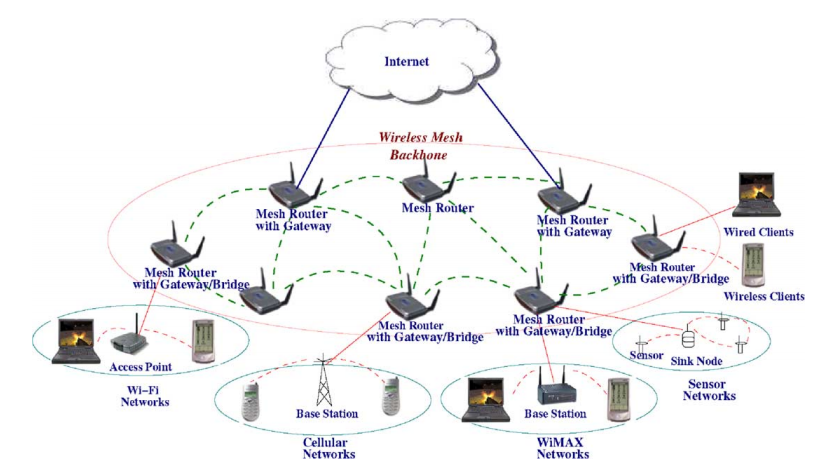
\includegraphics[scale=0.75]{infrastructure-mesh-clear.png}
\caption{Infrastructure/Backbone WMN}
\end{figure}

Infrastructure/Backbone WMNs are the most commonly used type. For example,
community and neighborhood networks can be built using infrastructure meshing.
The mesh routers are placed on the roofs of houses in a neighborhood, and these
can serve as access points for users in homes and along the roads. Typically, two
types of radio are used in the routers, i.e., for backbone communication and for user
communication. The mesh backbone communication can be established using long-
range communication techniques including, for example, directional antennas.
\subsubsection{Client WMNs}
Client meshing provides peer-to-peer networks among client devices.
In this type of architecture, client nodes constitute the actual network to perform
routing and configuration functionalities as well as providing end-user applications to
customers. Hence, a mesh router is not required for this type of network.
\begin{figure}[hbtp]
\centering
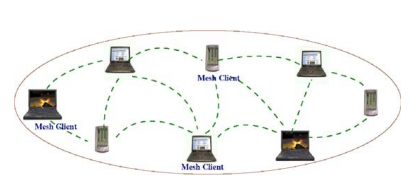
\includegraphics[scale=1]{client-wmn.png}
\caption{Client WMNs}
\end{figure}


\subsubsection{Hybrid WMNs}
This architecture is the combination of infrastructure and client
meshing. Mesh clients can access the network through mesh
routers as well as directly meshing with other mesh clients. While the infrastructure
provides connectivity to other networks such as the Internet, Wi-Fi, WiMAX, cellular,
and sensor networks, the routing capabilities of clients provide improved connectivity
and coverage inside the WMN.
\begin{figure}[hbtp]
\centering
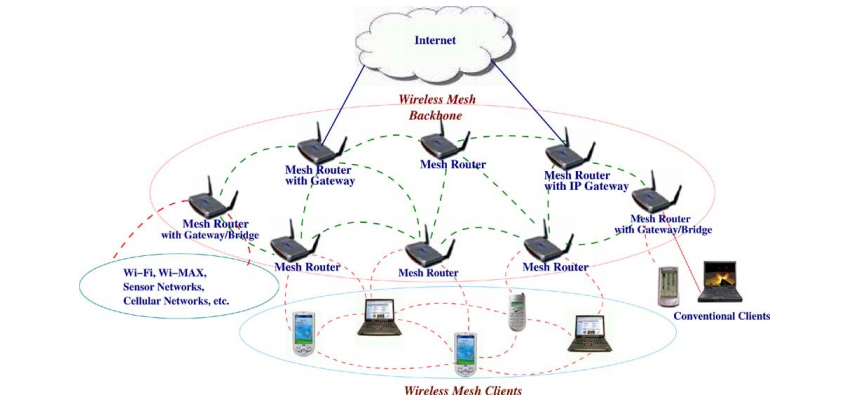
\includegraphics[scale=0.75]{hybrid-wmn.png}
\caption{Hybrid WMNs}
\end{figure}


%\subsection{Management}
%\subsection{Operation}

\subsection{Application}
Research and development of WMNs is motivated by several applications which clearly
demonstrate the promising market, but, at the same time, these applications cannot be
supported directly by other wireless networks such as cellular systems, ad hoc networks,
wireless sensor networks, standard IEEE 802.11, etc. In this section, we discuss these
applications.
\begin{itemize}
\item Broadband home networking
\item Community and neighborhood networking
\item Enterprise networking
\item Metropolitan area networks (MAN)
\item Transportation systems
\item Building automation
\item Health and medical systems
\item Security surveillance systems
\end{itemize}
In addition to the above applications, WMNs can also be applied to spontaneous
(emergency/disaster) networking and P2P communications. For example, wireless networks
for an emergency response team and firefighters do not have in-advance knowledge of
where the network should be deployed. By simply placing wireless mesh routers in
desired locations, a WMN can be quickly established.
For a group of people holding
devices with wireless networking capability, e.g., laptops and PDAs, P2P communication
anytime anywhere is an efficient solution for information sharing. WMNs are able to meet this demand. These applications illustrate that WMNs are a superset of ad hoc networks, and
thus, can accomplish all functions provided by ad hoc networking.

\section{Routing Protocols}
WMNs will be tightly integrated with the Internet, and IP has been accepted as a network layer protocol for many wireless networks including WMNs. However, routing protocols for WMNs are different from those in wired networks and cellular networks. Therefore, we focus our study on routing protocols in this section.
Since WMNs share common features with adhoc networks, the routing protocols developed for ad hoc networks can be applied to WMNs.
\subsection{Destination Source Routing Protocol (DSR)}
\subsection{Destination Sequence Distance Vector Routing Protocol (DSDV)}
\subsection{Adhoc On-demand Distance Vector Routing Protocol (AODV)}
\subsection{Hybrid Wireless Mesh Protocol (HWMP)}
\subsection{Optimized Link State Routing Protocol (OLSR)}

%\subsubsection{Broadband Home Networking}
%\subsubsection{Community and Neighborhood Networking}
%\subsubsection{Enterprise Networking}
%\subsubsection{Metropolitan Area Networks (MAN)}
%\subsubsection{Transportation Systems}
%\subsubsection{Building Automation}
%\subsubsection{Health and Medical Systems}
%\subsubsection{Transportation Systems}
%\subsubsection{Security Surveillance Systems}

%\section{Handoff Management}
%\subsection{Types of Handoff in Wireless Mesh Network Systems}
%\subsubsection{Intra-system Handoff}
%\subsubsection{Inter-system Handoff}
%\subsubsection{Hard Handoff}
%\subsubsection{Soft Handoff}

%\newpage
%\subsection{Conditions of Handoff}
%\subsection{Objectives of Handoff}
%\subsection{Types of Handoff}
%\subsubsection{Link Layer Handoff}
%\subsubsection{Network Layer Handoff}

\section{Related Work}

\chapter{Methodology}
\section{Existing Approaches}
%\subsection{Routing Based Location Update}
%\section{Multihash Location Management}
\section{Existing Methodology }
\section{Improved Methodology}

\chapter{Implementation}
\section{IEEE 802.11 standard}

\section{IEEE 802.11s}
\subsection*{Description}
\section{802.11 Mesh Architecture}
\subsection*{Routing Protocols}
\section{Network Simulator}
\subsection{ns-1}
\subsection{ns-2}
\subsection{ns-3}
\section{IEEE 802.11s Model in ns-3}
\section{Network Simulator 3}
\subsection{Model Design}
\subsubsection{Supported Features}
\subsubsection{Unsupported Features}
\subsection{Model Implementation}
\subsection{MAC Layer Routing Model}
\section{Simulation Environment}
\section{Simulation Visualization}

\chapter{Experimental Results and Discussion}
\section{Simulation Output }
\subsection{Comparison with Traditional Handoff}
\section{Trace Data Analysis}
\section{Result Analysis}
\subsection{Average End-to-End Delay Vs Simulation Time Delay for TCP}
\subsection{Average End-to-End Delay Vs Simulation Time Delay for UDP}
\subsection{Average Packet Delivery Ratio Vs Simulation Time for TCP}
\subsection{Average Packet Delivery Ratio Vs Simulation Time for UDP}

\chapter{Conclusion}
\section{Conclusion}
\section{Future Improvements}














\end{document}